\chapter{AFABL in Context}\label{ch:afabl-context}

In this chapter we place AFABL in context. First we present an extended example that compares typical AFABL code to typical Scala code for a series of agent programs for increasingly complex but closely related task environments. This example demonstrates the sub-linear progression of complexity of AFABL code compared to a linear progression of complexity for traditional code on the same task progression. Finally we discuss the kinds of problems that are well-suited to AFABL and those that are not well-suited to AFABL.

\section{AFABL Programs versus Traditional Programs}

In this section we incrementally expand the Bunny world from previous chapters to show how AFABL programs and traditional programs grow in response to additional world dynamics. The sections below show typical submissions from the previous chapter and build on them using similar styles to handle increasingly complex world dynamics. These examples demonstrate the superior scalability of AFABL.

\subsection{Bunny, Food}

To help keep the code straight, we will number each task starting at 0. We start with the simplest task, that of finding food. Figure \ref{fig:afabl0} shows the AFABL agent for Task 0.

\begin{figure}[h]
\begin{lstlisting}[language=Scala]
object AfablTask0 {
  case class FindFoodState(bunny: Location, food: Location)

  val findFood = AfablModule(
    world = bunnyWorld,
    stateAbstraction = (worldState: BunnyState) => {
      FindFoodState(worldState.bunny, worldState.food)
    },
    moduleReward = (moduleState: FindFoodState) => {
      if (moduleState.bunny == moduleState.food) 1.0
      else -0.1
    }
  )

  val afablBunny0 = AfablAgent(

    world = bunnyWorld,

    modules = Seq(findFood),

    agentLevelReward = (state: BunnyState) => {
      if (world.bunnyEats()) 1.0
      else 0.5
    }
  )
}
\end{lstlisting}
\caption{An AFABL bunny agent that finds food.}
\label{fig:afabl0}
\end{figure}

Figure  \ref{fig:scala0} shows the Scala code for Task 0.

\begin{figure}[h]
\begin{lstlisting}[language=Scala]
class ScalaBunny0 extends Agent[BunnyState, BunnyAction.Value] {

  def getAction(state: BunnyState) = {
      moveTowardFood(state)
   }

  def moveTowardFood(state: BunnyState) = {
    if (state.food.x > state.bunny.x)
      BunnyAction.Right
    else if (state.food.x < state.bunny.x)
      BunnyAction.Left
    else if (state.food.y < state.bunny.y)
      BunnyAction.Up
    else
      BunnyAction.Down
  }
}
\end{lstlisting}
\caption{A Scala bunny agent that finds food.}
\label{fig:scala0}
\end{figure}


\subsection{Bunny, Food, Wolf}

Task 1 adds the task of avoiding a wolf. As we see in Figure \ref{fig:afabl1}, the AFABL version looks quite similar -- we simply add a module with a different state abstraction and reward function, and incorporate the added criterion of avoiding the wolf to the agent level reward.

\begin{figure}[h]
\begin{lstlisting}[language=Scala]
object AfablTask1 {
  case class FindFoodState(bunny: Location, food: Location)
  case class AvoidWolfState(bunny: Location, wolf: Location)

  val avoidWolf = AfablModule(
    world = bunnyWorld,
    stateAbstraction = (worldState: BunnyState) => {
      AvoidWolfState(worldState.bunny, worldState.wolf)
    },
    moduleReward = (moduleState: AvoidWolfState) => {
      if (moduleState.bunny == moduleState.wolf) -0.1
      else 0.1
    }
  )

  val afablBunny1 = AfablAgent(

    world = bunnyWorld,

    modules = Seq(AfablTask0.findFood, avoidWolf),

    agentLevelReward = (state: BunnyState) => {
      if (world.bunnyDies()) 0.0
      else if (world.bunnyEats()) 1.0
      else 0.5
    }
  )
}
\end{lstlisting}
\caption{An AFABL bunny agent that finds food and avoids a wolf.}
\label{fig:afabl1}
\end{figure}

Figure  \ref{fig:scala1} shows the Scala code for Task 1, which adds logic for analyzing the relative distance of the wolf to the food in order to choose between pursuing food or runing away from the wolf.

\begin{figure}[h]
\begin{lstlisting}[language=Scala]
class ScalaBunny1 extends Agent[BunnyState, BunnyAction.Value] {

  def getAction(state: BunnyState) = {
    if (wolfNearFood(state))
      moveAwayFromWolf(state)
    else
      moveTowardFood(state)
   }

  def wolfNearFood(state: BunnyState) = {
    val wolfToFood = sqrt(pow(state.food.x - state.wolf.x, 2) +
                          pow(state.food.y - state.wolf.y, 2))
    val bunnyToFood = sqrt(pow(state.food.x - state.bunny.x, 2) +
                           pow(state.food.y - state.bunny.y, 2))
    wolfToFood < bunnyToFood
  }

  def moveTowardFood(state: BunnyState) = {
    if (state.food.x > state.bunny.x)
      BunnyAction.Right
    else if (state.food.x < state.bunny.x)
      BunnyAction.Left
    else if (state.food.y < state.bunny.y)
      BunnyAction.Up
    else
      BunnyAction.Down
  }

  def moveAwayFromWolf(state: BunnyState) = {
    if (state.wolf.x < state.bunny.x)
      BunnyAction.Right
    else if (state.wolf.x > state.bunny.x)
      BunnyAction.Left
    else if (state.wolf.y > state.bunny.y)
      BunnyAction.Up
    else
      BunnyAction.Down
  }
}
\end{lstlisting}
\caption{A Scala bunny agent that finds food and avoids a wolf.}
\label{fig:scala1}
\end{figure}

\subsection{Bunny, Food, Wolf, Mate}

Task 2 adds the task of finding a mate. The AFABL agent is able to reuse modules from afablBunny1 directly. ScalaBunny2 also benefits from the refactoring of common logic in ScalaBunny1.

\begin{figure}[h]
\begin{lstlisting}[language=Scala]
object AfablTask2 {
  case class FindFoodState(bunny: Location, food: Location)
  case class AvoidWolfState(bunny: Location, wolf: Location)
  case class FindMateState(bunny: Location, mate: Location)

  val findMate = AfablModule(
    world = bunnyWorld,
    stateAbstraction = (state: BunnyState) => {
      FindMateState(state.bunny, state.mate)
    },
    moduleReward = (state: FindMateState) => {
      if (world.bunnyMates()) 1.0
      else -0.1
    }
  )

  val afablBunny2 = AfablAgent(

    world = bunnyWorld,

    modules = Seq(AfablTask0.findFood, AfablTask1.avoidWolf, findMate),

    agentLevelReward = (state: BunnyState) => {
      if (world.bunnyDies()) 0.0
      else if (world.bunnyEats()) 1.0
      else if (world.bunnyMates()) 1.0
      else 0.5
    }
  )
}
\end{lstlisting}
\caption{An AFABL bunny agent that finds food, avoids a wolf, and pursues a mate.}
\label{fig:scala2}
\end{figure}

In ScalaBunny2, shown in Figure \ref{fig:scala2}, we follow the advice of Martin Fowler: if you need the same code in two places, copy and paste. If you need the same code in a third place, refactor the common logic in reusable program units. In ScalaBunny2 we factor out the code for finding distance and the code for moving towards something.

\begin{figure}[h]
\begin{lstlisting}[language=Scala]
class ScalaBunny2 extends Agent[BunnyState, BunnyAction.Value] {

  def getAction(state: BunnyState) = {
    if ((distance(state.wolf, state.food) < distance(state.food, state.bunny))
      || distance(state.wolf, state.mate) < distance(state.mate, state.bunny))
      moveAwayFromWolf(state)
    else if (distance(state.bunny, state.food) < distance(state.bunny, state.mate))
      moveToward(state.bunny, state.food)
    else
      moveToward(state.bunny, state.mate)
  }

  def distance(a: Location, b: Location) = {
    sqrt(pow(a.x - b.x, 2) + pow(a.y - b.y, 2))
  }

  def moveToward(from: Location, to: Location) = {
    if (to.x > from.x)
      BunnyAction.Right
    else if (to.x < from.x)
      BunnyAction.Left
    else if (to.y > from.y)
      BunnyAction.Up
    else
      BunnyAction.Down
  }

  def moveAwayFromWolf(state: BunnyState) = {
    if (state.wolf.x < state.bunny.x)
      BunnyAction.Right
    else if (state.wolf.x > state.bunny.x)
      BunnyAction.Left
    else if (state.wolf.y > state.bunny.y)
      BunnyAction.Up
    else
      BunnyAction.Down
  }
}
\end{lstlisting}
\caption{A Scala bunny agent that finds food, avoids a wolf, and finds a mate.}
\label{fig:scala2}
\end{figure}

\subsection{Bunny, Wolf, Food, Mate, Spoiling Food}

Task 3 adds spoilage to the food. If the bunny does not eat the food within {\tt SPOIL\_TIME} time steps the food disappears and new food respawns elsewhere. Here we begin to see the scalability benefits of AFABL. As we see in Figure \ref{fig:afabl3}, adapting afablBunny2 to Task 3 requires no new code whatsoever. The reinforcement learning algorithms underlying the AFABL code adjust to the new world dynamics automatically. The Scala version, on the other hand, adds a tremendous amount of logic to add consideration of spoiling food.

\begin{figure}[h]
\begin{lstlisting}[language=Scala]
object AfablTask3 {
  val afablBunny3 = AfablAgent(

    world = bunnyWorld,

    modules = Seq(AfablTask0.findFood, AfablTask1.avoidWolf, AfablTask2.findMate),

    agentLevelReward = (state: BunnyState) => {
      if (world.bunnyDies()) 0.0
      else if (world.bunnyEats()) 1.0
      else if (world.bunnyMates()) 1.0
      else 0.5
    }
  )
}
\end{lstlisting}
\caption{An AFABL bunny agent that finds food that spoils, avoids a wolf, and finds a mate.}
\label{fig:afabl3}
\end{figure}

Figure  \ref{fig:scala3} shows the Scala code for Task 3. ScalaBunny3 extends ScalaBunny2 to inherit its distance and moveTowards methods, but we must add logic to determine when it doesn't make sense to move towards the food because it will spoil before the bunny gets to it. This is a fairly straightforward approach but required some thought to come up with and the resulting code is slightly more complex due to the additional predicates in decision structures.

\begin{figure}[h]
\begin{lstlisting}[language=Scala]
class ScalaBunny3 extends ScalaBunny2 {

  val SPOIL_TIME = 10
  var stepCount = 0

  override def getAction(state: BunnyState) = {
    stepCount = stepCount + 1
    if ((distance(state.wolf, state.food) < distance(state.food, state.bunny))
      || distance(state.wolf, state.mate) < distance(state.mate, state.bunny))
      moveAwayFromWolf(state)
    else if (distance(state.bunny, state.food) < distance(state.bunny, state.mate)
      && distance(state.bunny, state.food) < stepCount % SPOIL_TIME)
      moveToward(state.bunny, state.food)
    else
      moveToward(state.bunny, state.mate)
  }

  def moveAwayFromWolf(state: BunnyState) = {
    if (state.wolf.x < state.bunny.x)
      BunnyAction.Right
    else if (state.wolf.x > state.bunny.x)
      BunnyAction.Left
    else if (state.wolf.y > state.bunny.y)
      BunnyAction.Up
    else
      BunnyAction.Down
  }
}
\end{lstlisting}
\caption{A Scala bunny agent that finds food that spoils, avoids a wolf, and finds a mate.}
\label{fig:scala3}
\end{figure}


\subsection{Bunny, Food, Wolf, Mate, Spoiling Food, Picky Mate}

Task 4 adds a picky mate that won't mate unless the bunny has eaten within the last {\tt HUNGER\_LIMIT} time steps. Here again we see that no new code needs to be written for the AFABL agent in Figure \ref{fig:afabl4}. The reinforcement learning algorithms simply learns new behavior for the changing world dynamics.

\begin{figure}[h]
\begin{lstlisting}[language=Scala]
object AfablTask4 {
  val afablBunny4 = AfablAgent(

    world = bunnyWorld,

    modules = Seq(AfablTask0.findFood, AfablTask1.avoidWolf, AfablTask2.findMate),

    agentLevelReward = (state: BunnyState) => {
      if (world.bunnyDies()) 0.0
      else if (world.bunnyEats()) 1.0
      else if (world.bunnyMates()) 1.0
      else 0.5
    }
  )
}
\end{lstlisting}
\caption{An AFABL bunny agent that finds food that spoils, avoids a wolf, and finds a mate who rejects the bunny if the bunny hasn't eaten recently.}
\label{fig:afabl4}
\end{figure}

ScalaBunny4, shown in Figure \ref{fig:scala4}, requires much more logic than ScalaBunny3. ScalaBunny4 must keep a reference to the world to know when it has eaten, it must keep track of its hunger level, and the decision of whether to pursue the food or the mate is now more complicated.

\begin{figure}[h]
\begin{lstlisting}[language=Scala]
class ScalaBunny4(val world: BunnyWorld) extends ScalaBunny3 {

  val HUNGER_LIMIT
  val SPOIL_TIME = 10
  var stepCount = 0
  var hungerLevel = 0

  override def getAction(state: BunnyState) = {
    stepCount = stepCount + 1
    if (world.bunnyEats()) {
      hungerLevel = 0
    } else {
      hungerLevel = hungerLevel + 1
    }
    if ((distance(state.wolf, state.food) < distance(state.food, state.bunny))
      || distance(state.wolf, state.mate) < distance(state.mate, state.bunny))
      moveAwayFromWolf(state)
    else if ((distance(state.bunny, state.food) < distance(state.bunny, state.mate)
      && distance(state.bunny, state.food) < stepCount % SPOIL_TIME)
      || (hungerLevel + distance(state.bunny, state.mate) > HUNGER_LIMIT)
      moveToward(state.bunny, state.food)
    else
      moveToward(state.bunny, state.mate)
  }

  def moveAwayFromWolf(state: BunnyState) = {
    if (state.wolf.x < state.bunny.x)
      BunnyAction.Right
    else if (state.wolf.x > state.bunny.x)
      BunnyAction.Left
    else if (state.wolf.y > state.bunny.y)
      BunnyAction.Up
    else
      BunnyAction.Down
  }
}
\end{lstlisting}
\caption{A Scala bunny agent that finds food that spoils, avoids a wolf, and finds a mate who rejects the bunny if the bunny hasn't eaten recently.}
\label{fig:scala4}
\end{figure}

\subsection{Analysis}

\begin{figure}[h!]
\begin{center}
  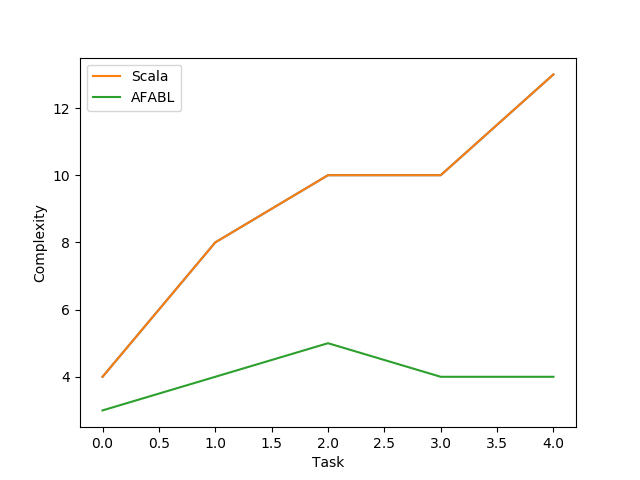
\includegraphics[height=3.5in]{complexity.png}
\end{center}
\caption{Growth in complexity of agent programs as the task becomes more complex.}
\label{fig:complexity}
\end{figure}

\begin{figure}[h!]
\begin{center}
  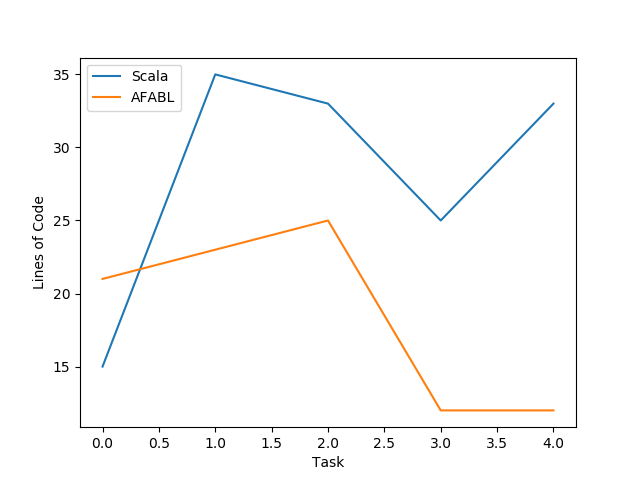
\includegraphics[height=3.5in]{loc.png}
\end{center}
\caption{Growth in lines of code in agent programs as the task becomes more complex.}
\label{fig:loc}
\end{figure}

Figure \ref{fig:complexity} shows the complexity of AFABL programs is lower than equivalent programs in traditional programming languages, that the complexity of AFABL code grows more slowly, and that once AFABL code has been written for the basic elements of a task environment, the complexity does not increases as the dynamics of the world change. In contrast, agent programs in traditional languages increase in complexity as the task environment increases in complexity in a linear fashion. The complexity of AFABL programs grows in a sub-linear, often logarithmic fashion when the task environment changes can be handled automatically by AFABL's reinforcement learning algorithms. We discuss this further in the next section.

In Figure \ref{fig:loc} we see a similar pattern in lines of AFABL code. The number of lines of code increases until the basic modules are defined, then the lines of code actually decrease as modules are reused. This reuse is one of the goals of AFABL. With the Scala code we see the benefit of refactoring code in traditional languages. While the Scala agents require far more code, the growth in lines of code slows as reusable functions are created. However, the complexity still grows due to the need to manually encode all the decision logic in the agent.


\section{When to Use AFABL}

AFABL shows the greatest scalability benefit when adapting agents to worlds with changing dynamics but the same state representation. As long as the state representation stays the same, the same AFABL code can be used in a world with different or changing dynamics. In fact, AFABL modules written separately with different reward structures can be used.

AFABL is a good choice for agent programs when:

\begin{itemize}
\item the agent pursue multiple subgoals simultaneously that are clearly separated and non-overlapping and thus can be modeled with behavior modules;
\item the subgoals are sometimes at odds, that is, when one two or more modules would choose to go in different directions;
\item there is an agent-level reward signal that represents goals that may or may not be represented in any module;
\item there is a single action set shared by all the modules; and
\item the world dynamics may change but retain the same state representation.
\end{itemize}

AFABL is not a good choice for all agent programs. In particular, AFABL is not a good choice when:
\begin{itemize}
\item the best action in some states is a compromise action, not the first choice of any module. In such cases AFABL's arbitration algorithm will choose a suboptimal action.
\item the agent's goals cannot be well modeled with concurrent subgoals;
\item there is no clear agent-level reward signal that can be used to automatically learn how to arbitrate modules' action choices; and
\item the problem itself is not well-suited to reinforcement learning agents in general.
\end{itemize}
